\documentclass{article}
\usepackage[margin=1.2in]{geometry}
\usepackage{datetime}
\usepackage{hyperref}      %for \url macro
\usepackage{microtype}     %attempt to fix issue with justification protrusion (in references)
\usepackage{amssymb}       % for formatting less/greater than symbols
\usepackage{amsmath}
\usepackage{enumitem}      %for changing spacing in bulleted lists
\usepackage{subfigure}        %for subfigures


\renewcommand{\arraystretch}{1.25}

\usepackage[gobble=auto, runall=true]{pythontex}
\usepackage{float} %for forcing position of images

\usepackage{graphicx}
\graphicspath{ {../images/} }
\usepackage[export]{adjustbox}
\usepackage[justification=centering]{caption}

\usepackage{listings}   %for typesetting code
\usepackage{color}
\definecolor{codegreen}{rgb}{0,0.6,0}
\definecolor{codegray}{rgb}{0.5,0.5,0.5}
\definecolor{codepurple}{rgb}{0.58,0,0.82}
\definecolor{backcolour}{rgb}{0.95,0.95,0.92}
\lstdefinestyle{mystyle}{
    backgroundcolor=\color{backcolour},
    commentstyle=\color{codegreen},
    keywordstyle=\color{codepurple},
    numberstyle=\tiny\color{codegray},
    stringstyle=\color{codepurple},
    basicstyle=\footnotesize,
    breakatwhitespace=false,
    breaklines=true,
    captionpos=b,
    keepspaces=true,
    %numbers=left,
    numbersep=5pt,
    showspaces=false,
    showstringspaces=false,
    showtabs=false,
    tabsize=2
}
\lstset{style=mystyle}

\frenchspacing                   %removes extra spacing after a period at the end of a sentence.
\newdateformat{daymonthyear}{\THEDAY\ \monthname\ \THEYEAR}

\title{CSC411 Machine Learning \\ Project 4: Reinforcement Learning}
\author{ Ariel Kelman \\ Student No: 1000561368
         \\ \\
         Gideon Blinick \\ Student No: 999763000 }
\daymonthyear



\begin{document}
   \maketitle{}


   \section{Introduction}
   \subsection{Results \& Report Reproducibility}
   All results and plots can be generated using the code in \texttt{tictactoe.py}.
   All code is python 3, run with Anaconda 3.6.3.
   Running the code will save all generated images in the \texttt{resources} folder,
   where they are used by \LaTeX. Note that some of the sections require the code for
   other sections (in the same file) to be run first.
   To reproduce the report, simply run it through \LaTeX. This will pull the most recently
   generated figures from the \texttt{resources} folder.

   \subsection{Tic Tac Toe Environment}
   The \texttt{Environment} class provides the functionality required to play a game of tic tac
   toe, including against an opponent who plays a random legal move. The game is represented by the
   \texttt{grid} attribute, which is a \texttt{numpy} array representing the $9$ positions. Each position
   can have a $0, 1$ or $2$, representing an empty position, or one filled by player 1 ($X$) or 2 ($O$)
   respectively. The \texttt{turn} attribute can have a value of $1$ or $2$, and represents which player
   has the next move. The \texttt{done} attribute is a boolean that indicates whether a game has been
   completed (either with a win, or when the board is full).

   The \texttt{step()} and \texttt{render()} methods allow a tic tac toe game to be played and displayed
   with text output. Using these methods, a game was played, resulting in the following output:
   \begin{lstlisting}[language=Python]

      ...
      .x.
      ...
      ====
      o..
      .x.
      ...
      ====
      o.x
      .x.
      ...
      ====
      o.x
      ox.
      ...
      ====
      o.x
      ox.
      x..
      ====
   \end{lstlisting}


   \section{Policy}
   The \texttt{Policy} class implements a neural network that learns to play tic tac toe. The provided
   starter code was modified to be a one-hidden layer neural network; the final code is shown in the
   code block below.
   \begin{lstlisting}[language=Python, label={PolicyClass}]

      class Policy(nn.Module):
         """
         The Tic-Tac-Toe Policy
         """
         def __init__(self, input_size=27, hidden_size=64, output_size=9):
              super().__init__()
              self.Linear1 = nn.Linear(input_size, hidden_size)
              self.Linear2 = nn.Linear(hidden_size, output_size)

         def forward(self, x):
              h = F.relu( self.Linear1(x) )
              out = F.softmax( self.Linear2(h) )
              return out
   \end{lstlisting}

   In choosing an action, the state is represented as a 27-dimensional vector, using a one-hot encoding
   type scheme. The first nine elements are $1$ if the corresponding location (moving horizontally, and then
   from top to bottom), and $0$ otherwise. Similarly, the next $9$ elements are $1$ if an $X$ (representing
   player 1) is in the corresponding location; while the last nine elements provide the same functionality
   for $O$ (player 2).

   The policy outputs a nine-dimensional vector, which is a probability distribution that is sampled to choose
   the move for the policy. Thus the policy is stochastic - the \texttt{select\_action()} function samples this
   distribution to choose a move.


   \section{Policy Gradient}
   The \texttt{compute\_returns()} function computes the returns based on the reward at the end of a game.
   The following code block shows how the returns are calculated.
   \begin{lstlisting}[language=Python, label={returns}]

      def compute_returns(rewards, gamma=1.0):
         """
         Compute returns for each time step, given the rewards
         """
         k = len(rewards)
         rewards = np.array(rewards)
         gammas = np.array( [gamma**(i) for i in range(k) ] )
         G = [ sum( rewards[i:]*gammas[:k-i] ) for i in range(k) ]
         return G
   \end{lstlisting}

   The weights are updated on the conclusion of a game, though this means that the policy does not improve
   during a game (this is a minor cost considering how short the games are). For updates to the policy to have
   any meaning in the middle of the game, there would need to be rewards for intermediate states. This would
   require having a metric that evaluates a tic tac toe position. While this could be done in tic tac toe,
   it would be quite difficult in more complicated games, where it is not obvious how a position should be
   rewarded. Having rewards only at the end still improves the policy choices earlier in the game (if an early
   position leads to a win, that position will be wieghted more positively when propogating backwards).
   Thus updating the weights at the end of an episode provides a simple way to provide feedback and improve the
   policy.

   \section{Rewards}
   When originally setting the rewards (in the \texttt{get\_reward()} function), they were set as shown in
   table \ref{part4}.
      \begin{table}[h]
         \centering
         \renewcommand{\arraystretch}{1.5}

         \begin{tabular}{ p{7em}|l }
            \hline
            status     &     reward      \\
            \hline \hline
            VALID\_MOVE        &  1             \\
            INVALID\_MOVE      &  -10             \\
            WIN               &  15             \\
            TIE               &  3             \\
            LOSE              &  -1             \\
            \hline
         \end{tabular}

         \caption{ Original rewards (the \texttt{DONE} status was not give a reward). }
         \label{part4}
      \end{table}
   The logic behind these rewards was to follow an intuitive feeling for how much the above results
   are actually desired. This is somewhat arbitrary, but does represent a reasonable starting point.
   Thus a valid move should get a small positive reward, while an invalid one should
   be heavily penalized. A win is highly rewarded, a tie gets some reward for preventing a loss, while a
   loss is penalized (it would have been reasonable to start with a more negative penalty here too).
   The \texttt{DONE} status was not given a reward; that scenario is taken care of by the \texttt{TIE} status.

   However, while debugging during training, the rewards were set to much simpler values, and - since
   after the issues were resolved the win rate was quite high - the changed rewards were kept. These rewards
   were simply $+1$ for a win, and $-1$ for an invalid move.
   A side-effect of this scheme is that the average return is equivalent to the win rate.

   The final \texttt{get\_reward()} function is shown in the following code block.
   \begin{lstlisting}[language=Python, label={reward}]

      def get_reward(status):
         """Returns a numeric given an environment status."""
         return {
                  Environment.STATUS_VALID_MOVE  : 0,
                  Environment.STATUS_INVALID_MOVE: -1,
                  Environment.STATUS_WIN         : 1,
                  Environment.STATUS_TIE         : 0,
                  Environment.STATUS_LOSE        : 0
         }[status]
   \end{lstlisting}


   \section{Training}
   \subsection{Learning Curve}
   Figure \ref{fig:5a} shows
      \begin{figure}[h] \centering
          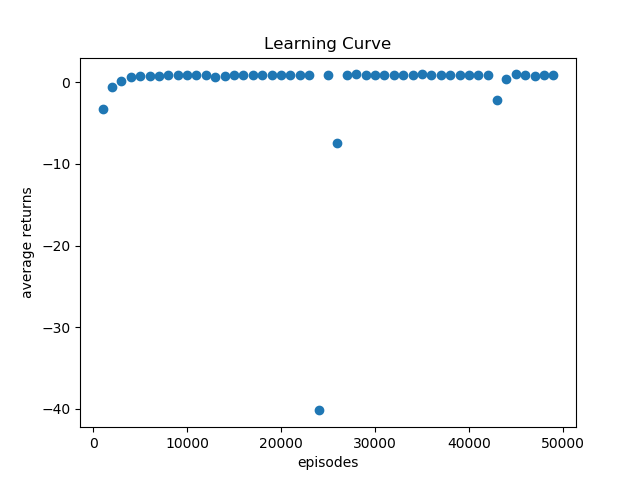
\includegraphics[width=4in]{resources/part5a}
          \caption{Learning curve. }
          \label{fig:5a}
       \end{figure}

   \subsection{Hidden Units}

   \subsection{Invalid Moves}
   Figure \ref{fig:5c} shows
      \begin{figure}[h] \centering
          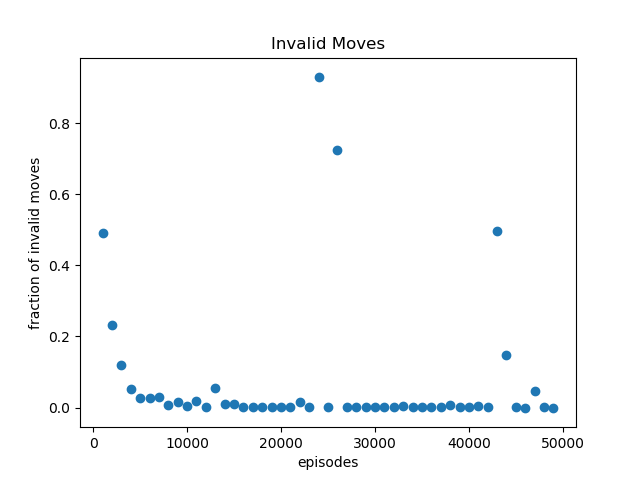
\includegraphics[width=4in]{resources/part5c}
          \caption{ Invalid moves. }
          \label{fig:5c}
       \end{figure}

   \subsection{Win-Lose-Tie Ratios}
   Playing 100 games against a randomized opponent...


   \section{Win Rate over Episodes}
   Figure \ref{fig:6} shows
      \begin{figure}[h] \centering
          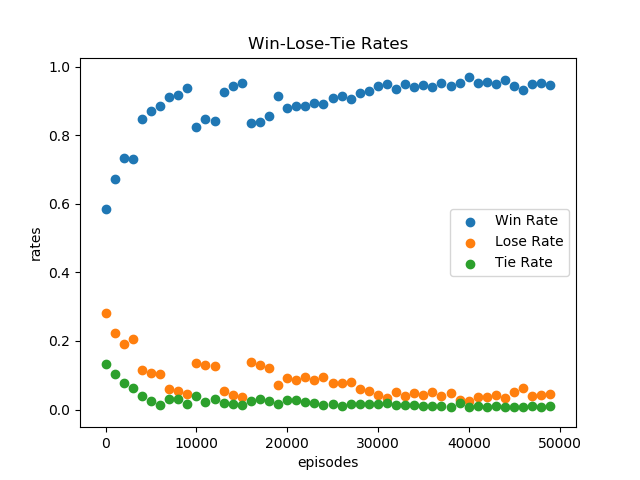
\includegraphics[width=4in]{resources/part6}
          \caption{ Win-Lose-Tie Ratios }
          \label{fig:6}
       \end{figure}


   \section{First Moves}
   \section{Limitations}


\end{document}
